\documentclass[a4paper]{scrartcl}
\usepackage{amsmath,amssymb,amsthm}
\usepackage{bm}
\usepackage{biblatex}
\usepackage{caption}
\usepackage{subcaption}
\usepackage{float}
\usepackage[colorlinks=true, allcolors = black, urlcolor=cyan]{hyperref}
\usepackage{graphicx}
\usepackage{mathtools}
\usepackage{matlab-prettifier}
\usepackage{physics}

\renewcommand{\thesection}{\arabic{section}}
\renewcommand{\thesubsection}{\alph{subsection}}

\title{Assignment 3}
\subtitle{TTK4210 - Advanced Control of Industrial Processes}
\author{Sondre Myrberg}
\date{\today}

\setlength{\parindent}{0pt} % Disable indentation
\mathtoolsset{showonlyrefs} % Only show equation numbers on referenced equations


\begin{document}

\hypersetup{pageanchor=false}
\begin{titlepage}
    \maketitle
    \vfill
    \vfill
    \vfill
    \vfill
    \vfill
    
\includegraphics[width=0.95\textwidth]{../ntnu_logo.pdf}
    \vfill
    \vfill
\end{titlepage}
\hypersetup{pageanchor=true}

\section{Anti-windup (and simulation) for the LV-model}
Using the provided solution from assignment 2.
\subsection{Implementation}
In the PI-controller we get the transfer functions
\begin{equation}
	\begin{aligned}
		k_1 &= \frac{s+\tfrac{1}{2}}{2s} = \frac{1}{2} \frac{2s+1}{2s}\\
		k_2 &= \frac{-s-\tfrac{1}{2}}{2s} = -\frac{1}{2} \frac{2s+1}{2s}
	\end{aligned}
\end{equation}
which yields the parameters
\begin{center}
	\begin{tabular}{c|c|c}
		$j$ & $1$ & $2$ \\ \hline
		$K_{p_j}$ & $\frac{1}{2}$ & $-\frac{1}{2}$\\
		$T_{i_j}$ & $2$ & $2$
	\end{tabular}
\end{center}
Using the anti-windup scheme for PI-controllers given in 6.3.1 in the course notes we can implement anti-windup as shown in \autoref{fig:1PIantiwindup} and \autoref{fig:1LQGantiwindup}. I don't have time and energy for the decoupled controller now.

\begin{figure}[ht!]
	\centering
	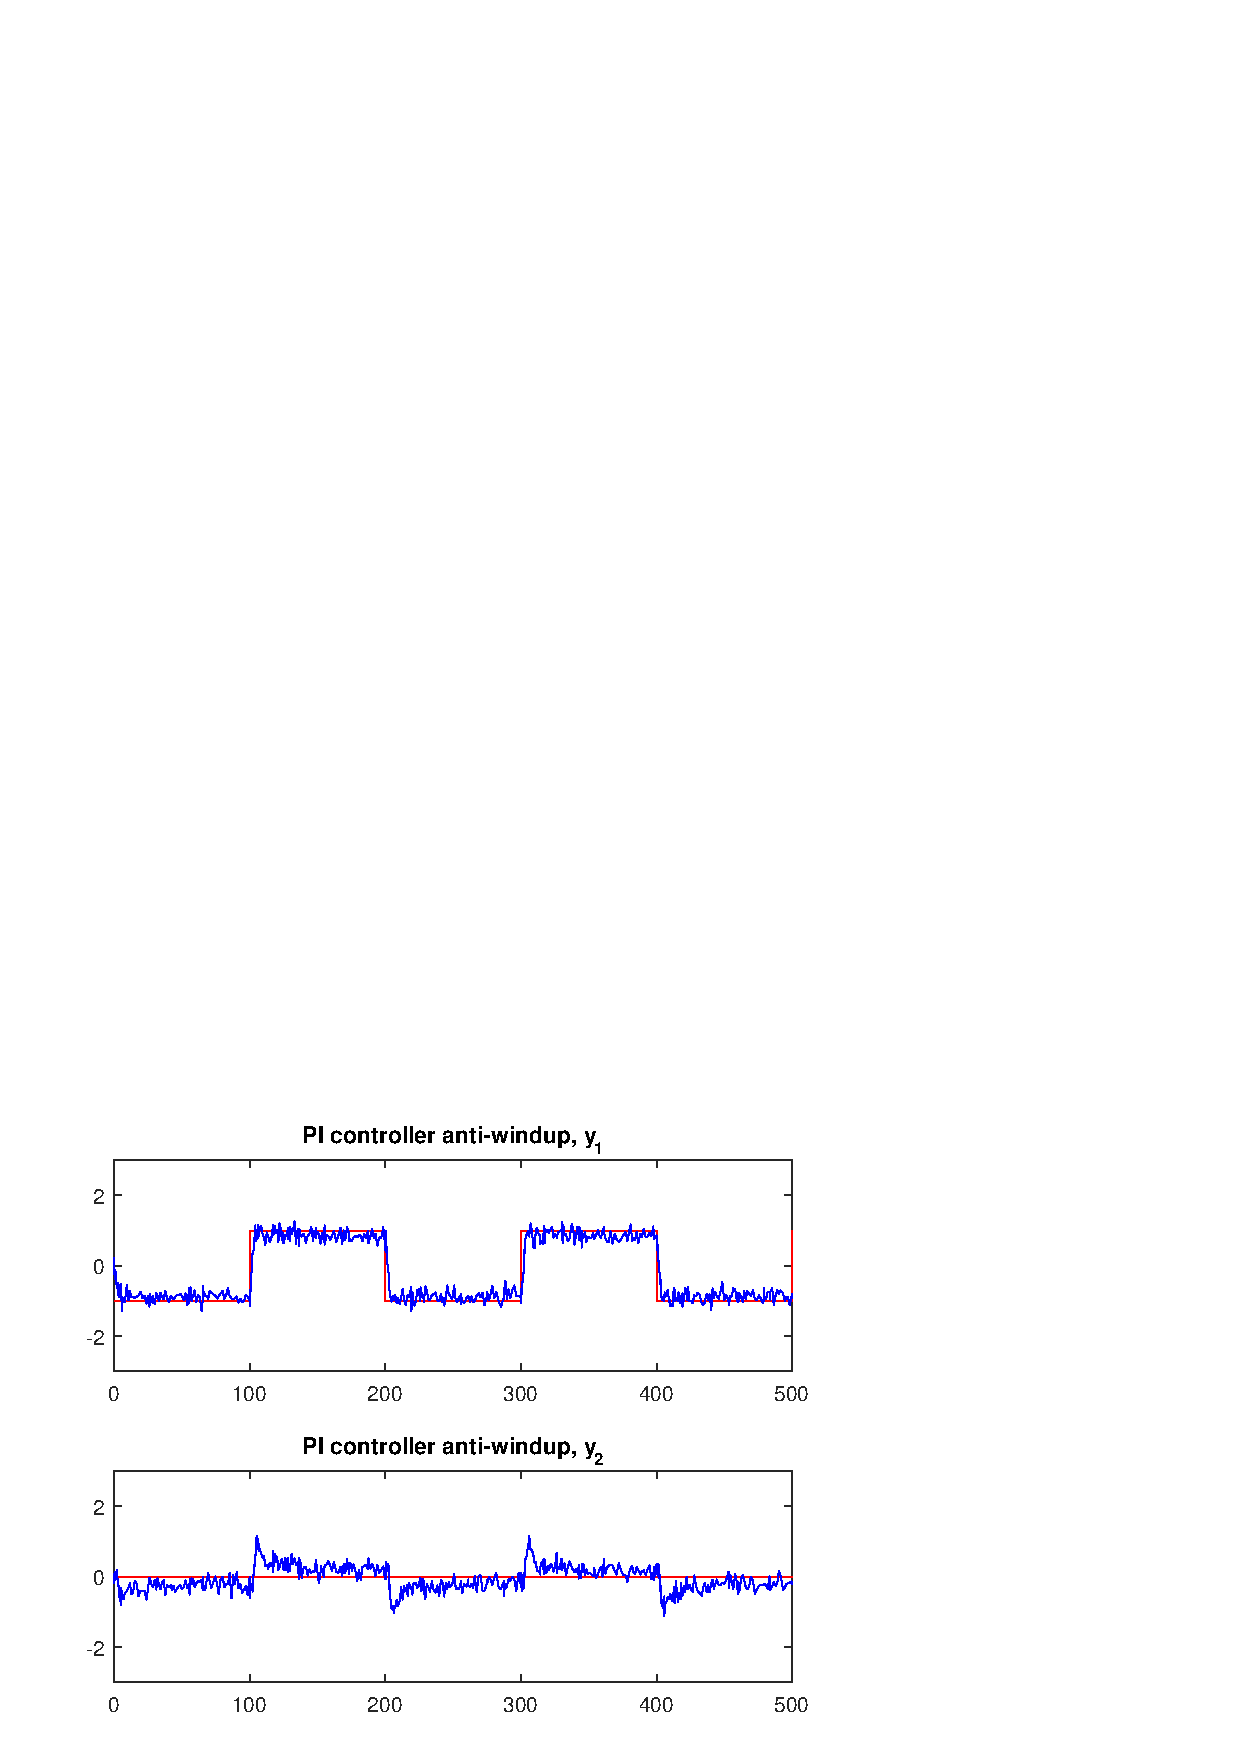
\includegraphics[width=0.95\textwidth]{fig/simulink/PI_antiwindup.pdf}
	\caption{Anti-windup for PI controller}
	\label{fig:1PIantiwindup}
\end{figure}
\begin{figure}[ht!]
	\centering
	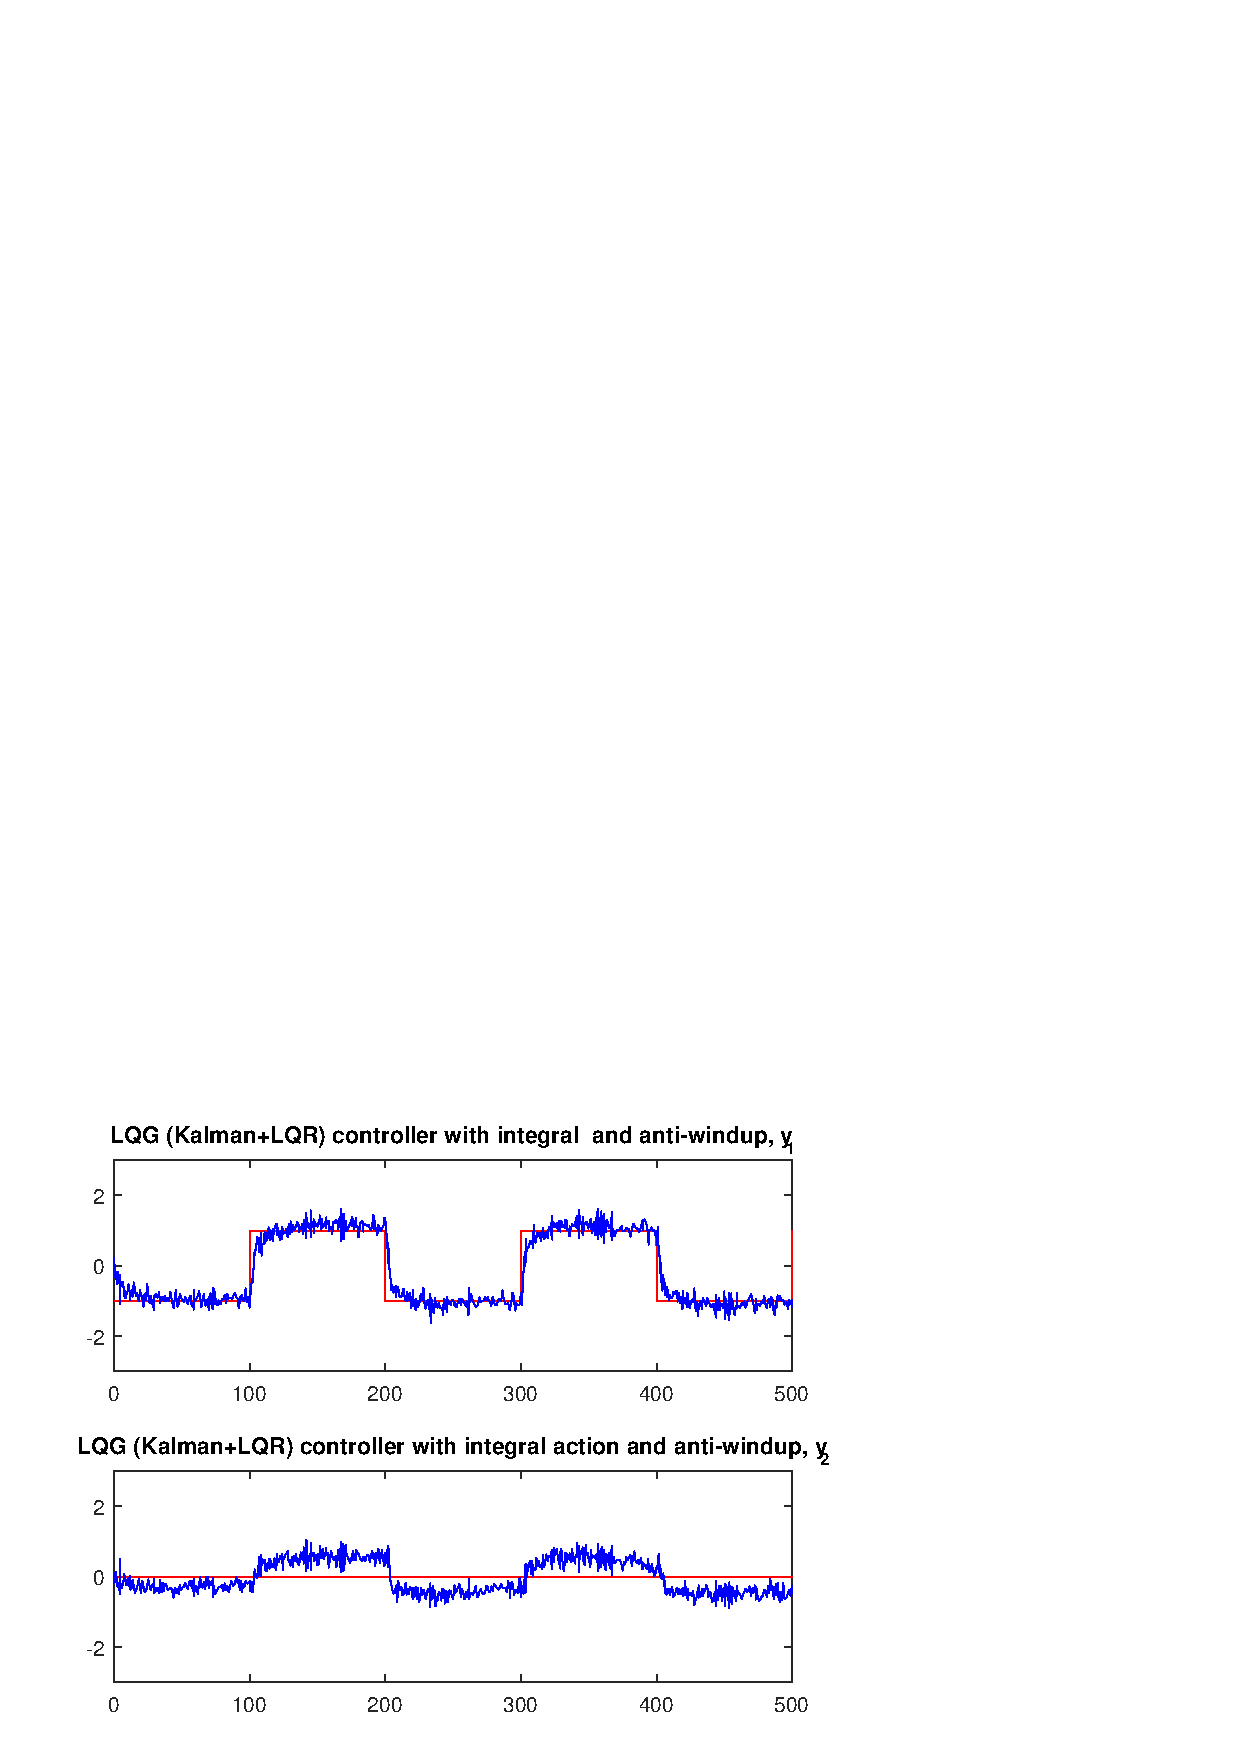
\includegraphics[width=0.95\textwidth]{fig/simulink/LQG_antiwindup.PDF}
	\caption{Anti-windup for LGQ-controller with integral action}
	\label{fig:1LQGantiwindup}
\end{figure}

\subsection{Simulation with anti-windup}
When simulating with and without anti-windup we clearly see differences in performance. The controllers with anti-windup implemented have smaller deviations from the setpoints than the controllers without anti-windup. For the PI-controller we see this in \autoref{fig:PIsim} and for the LQG-controller this is shown in \autoref{fig:LQGsim}. For both cases we see that the performance has increased significantly. 

\begin{figure}
\centering
\begin{subfigure}{.5\textwidth}
	\centering
	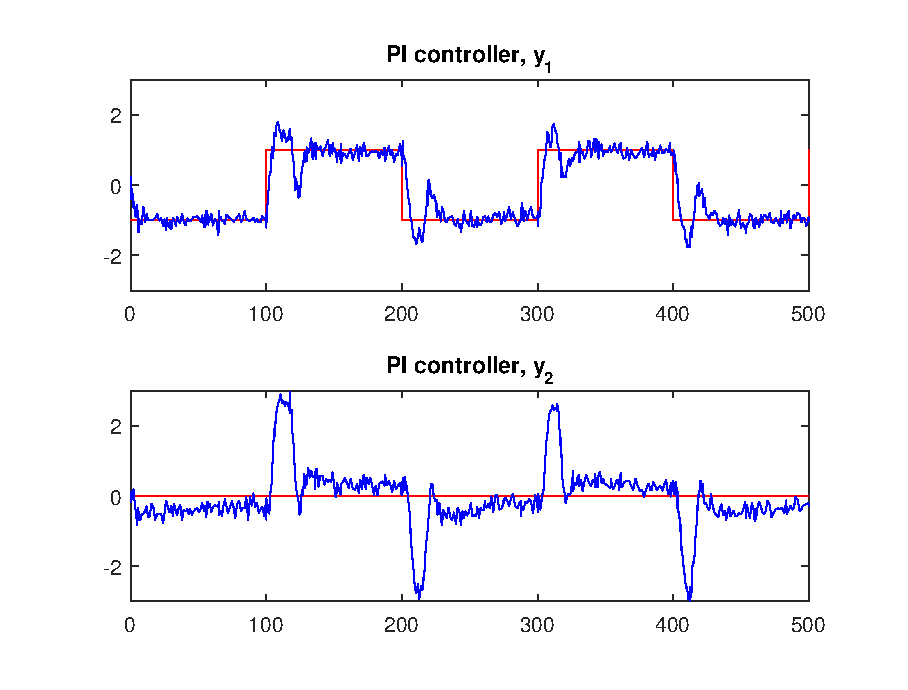
\includegraphics[width = .9\linewidth]{fig/task1/PI.eps}
	\caption{Simulation of the PI-controller without anti-windup}
	\label{fig:PIsimwithout}	
\end{subfigure}%
\begin{subfigure}{.5\textwidth}
	\centering
	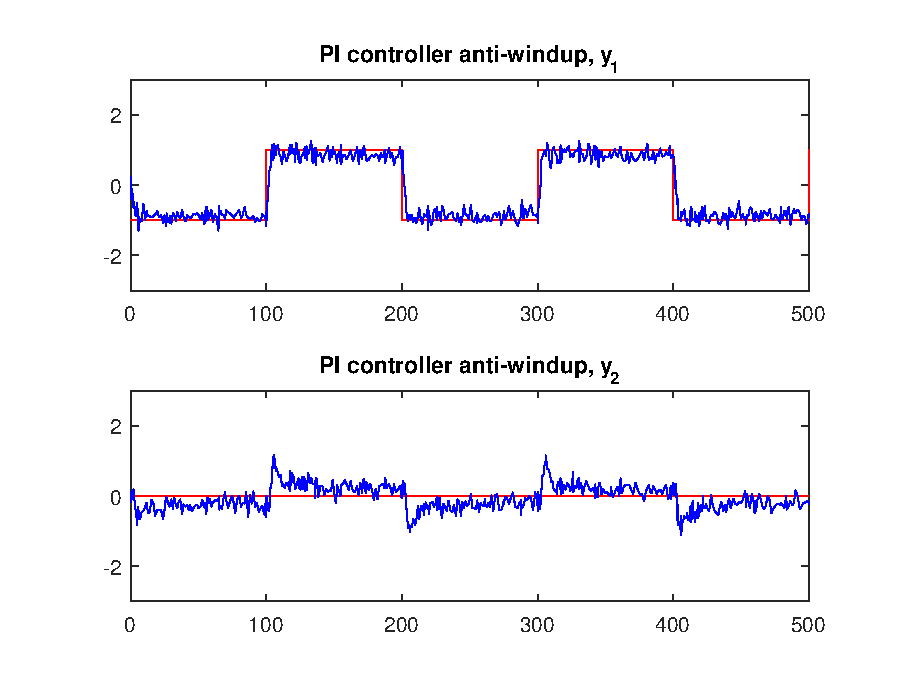
\includegraphics[width = .9\linewidth]{fig/task1/PI_antiwindup.eps}
	\caption{Simulation of the PI-controller with anti-windup}
	\label{fig:PIsimwith}	
\end{subfigure}
\caption{Comparison of the response of the PI-controller with and without anti-windup}
\label{fig:PIsim}
\end{figure}

\begin{figure}
\centering
\begin{subfigure}{.5\textwidth}
	\centering
	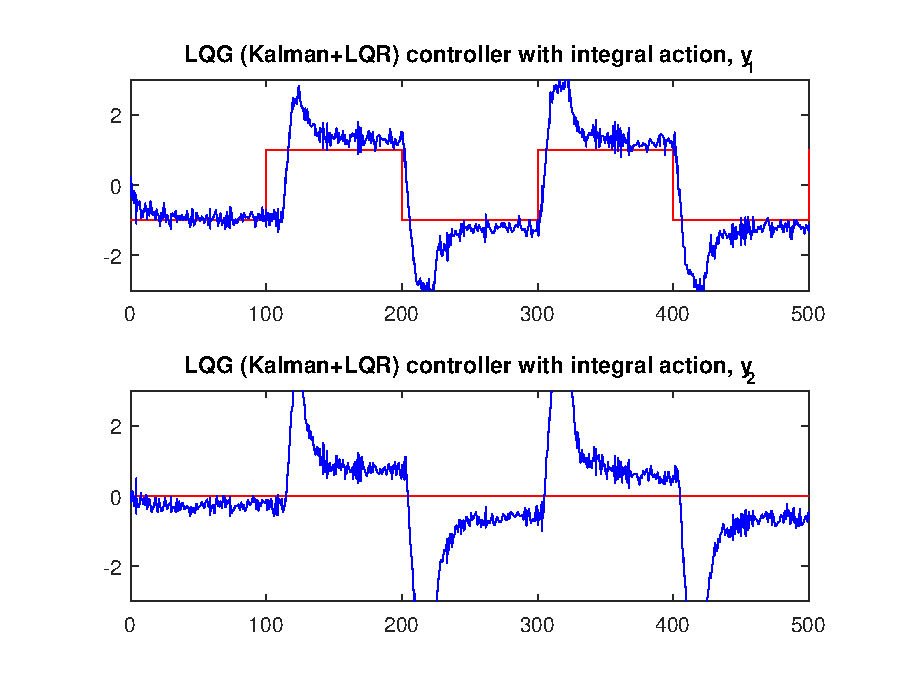
\includegraphics[width = .9\linewidth]{fig/task1/LQG.eps}
	\caption{Simulation of the LQG-controller without anti-windup}
	\label{fig:LQGsimwithout}	
\end{subfigure}%
\begin{subfigure}{.5\textwidth}
	\centering
	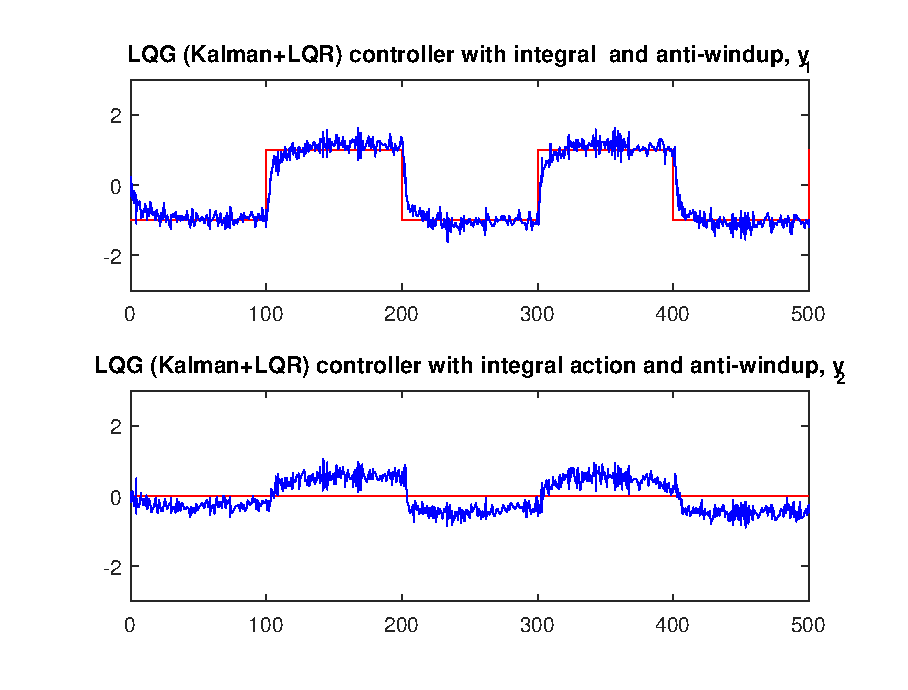
\includegraphics[width = .9\linewidth]{fig/task1/LQG_antiwindup.eps}
	\caption{Simulation of the LQG-controller with anti-windup}
	\label{fig:LQGsimwith}	
\end{subfigure}
\caption{Comparison of the response of the LQG-controller with and without anti-windup}
\label{fig:LQGsim}
\end{figure}

\clearpage
\section{Anti-windup with PI controllers and selectors}
\subsection{Model implementation}
The plant can be modelled as shown in \autoref{fig:2asystem} with $y(s) = G(s)u(s) + G_d(s)d(s)$.
\begin{figure}[ht!]
	\centering
	\includegraphics[width=0.9\textwidth]{fig/simulink/system.pdf}
	\caption{Implementation of the system given the transfer functions from input and disturbance to output}
	\label{fig:2asystem}
\end{figure}

\subsection{Controller tuning}
Using Ziegler-Nichols method of controlling a PI(D)-controller on each of the two control loops individually we get the following table of parameters

\begin{center}
	\begin{tabular}{c|c|c}
		Controller & $K_p$ & $T_i$ \\
		\hline
		Flow & $3.04$ & $4.63$\\
		Pressure & $18$ & $3.45$
	\end{tabular}
\end{center}
This was obtained by using a unit step function as disturbance and observing the corresponding outputs, as per Ziegler-Nichols method.

\subsection{Simulation without anti-windup}
The PI-controllers are implemented on the form shown in \autoref{fig:2PI}. Here we can manually choose between the regular PI-controller and the anti-windup PI-controller. The complete system is then shown in \autoref{fig:2csystem}. Here the selector chooses the output with lowest value. Simulating this yields the plot shown in \autoref{fig:2cwithout}. Here we see that only the pressure is controlled as the flow controller winds up and never gets low enough value to get chosen.

\begin{figure}[ht!]
	\centering
	\includegraphics[width=0.95\textwidth]{fig/simulink/PI_controller_task2_combined.pdf}
	\caption{Diagram of the flow controller both with and without anti-windup. The controller for pressure have the same exact form, but different values for $K$ and $T$.}
	\label{fig:2PI}
\end{figure}
\begin{figure}[ht!]
	\centering
	\includegraphics[width=0.95\textwidth]{fig/simulink/system_task2.pdf}
	\caption{Simulink diagram of the complete system with selector of lowest controller output implemented.}
	\label{fig:2csystem}
\end{figure}
\begin{figure}[ht!]
	\centering
	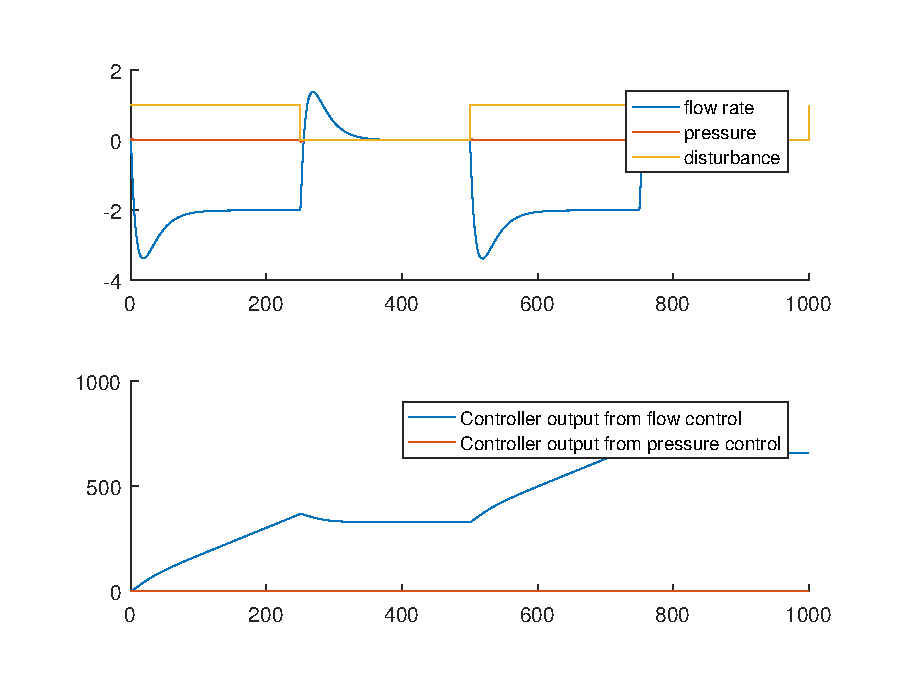
\includegraphics[width=0.9\textwidth]{fig/task2/2c_without_antiwindup.eps}
	\caption{System and controller output without anti-windup}
	\label{fig:2cwithout}
\end{figure}

\subsection{Simulation with anti-windup}

Simulating the same references and disturbances as abov, but choosing the anti-windup controller insted we get the response shown in \autoref{fig:2cwith}. Here we see that the selector choses the controller with the lowest output, thus both flow and pressure gets controlled.

\begin{figure}[ht!]
	\centering
	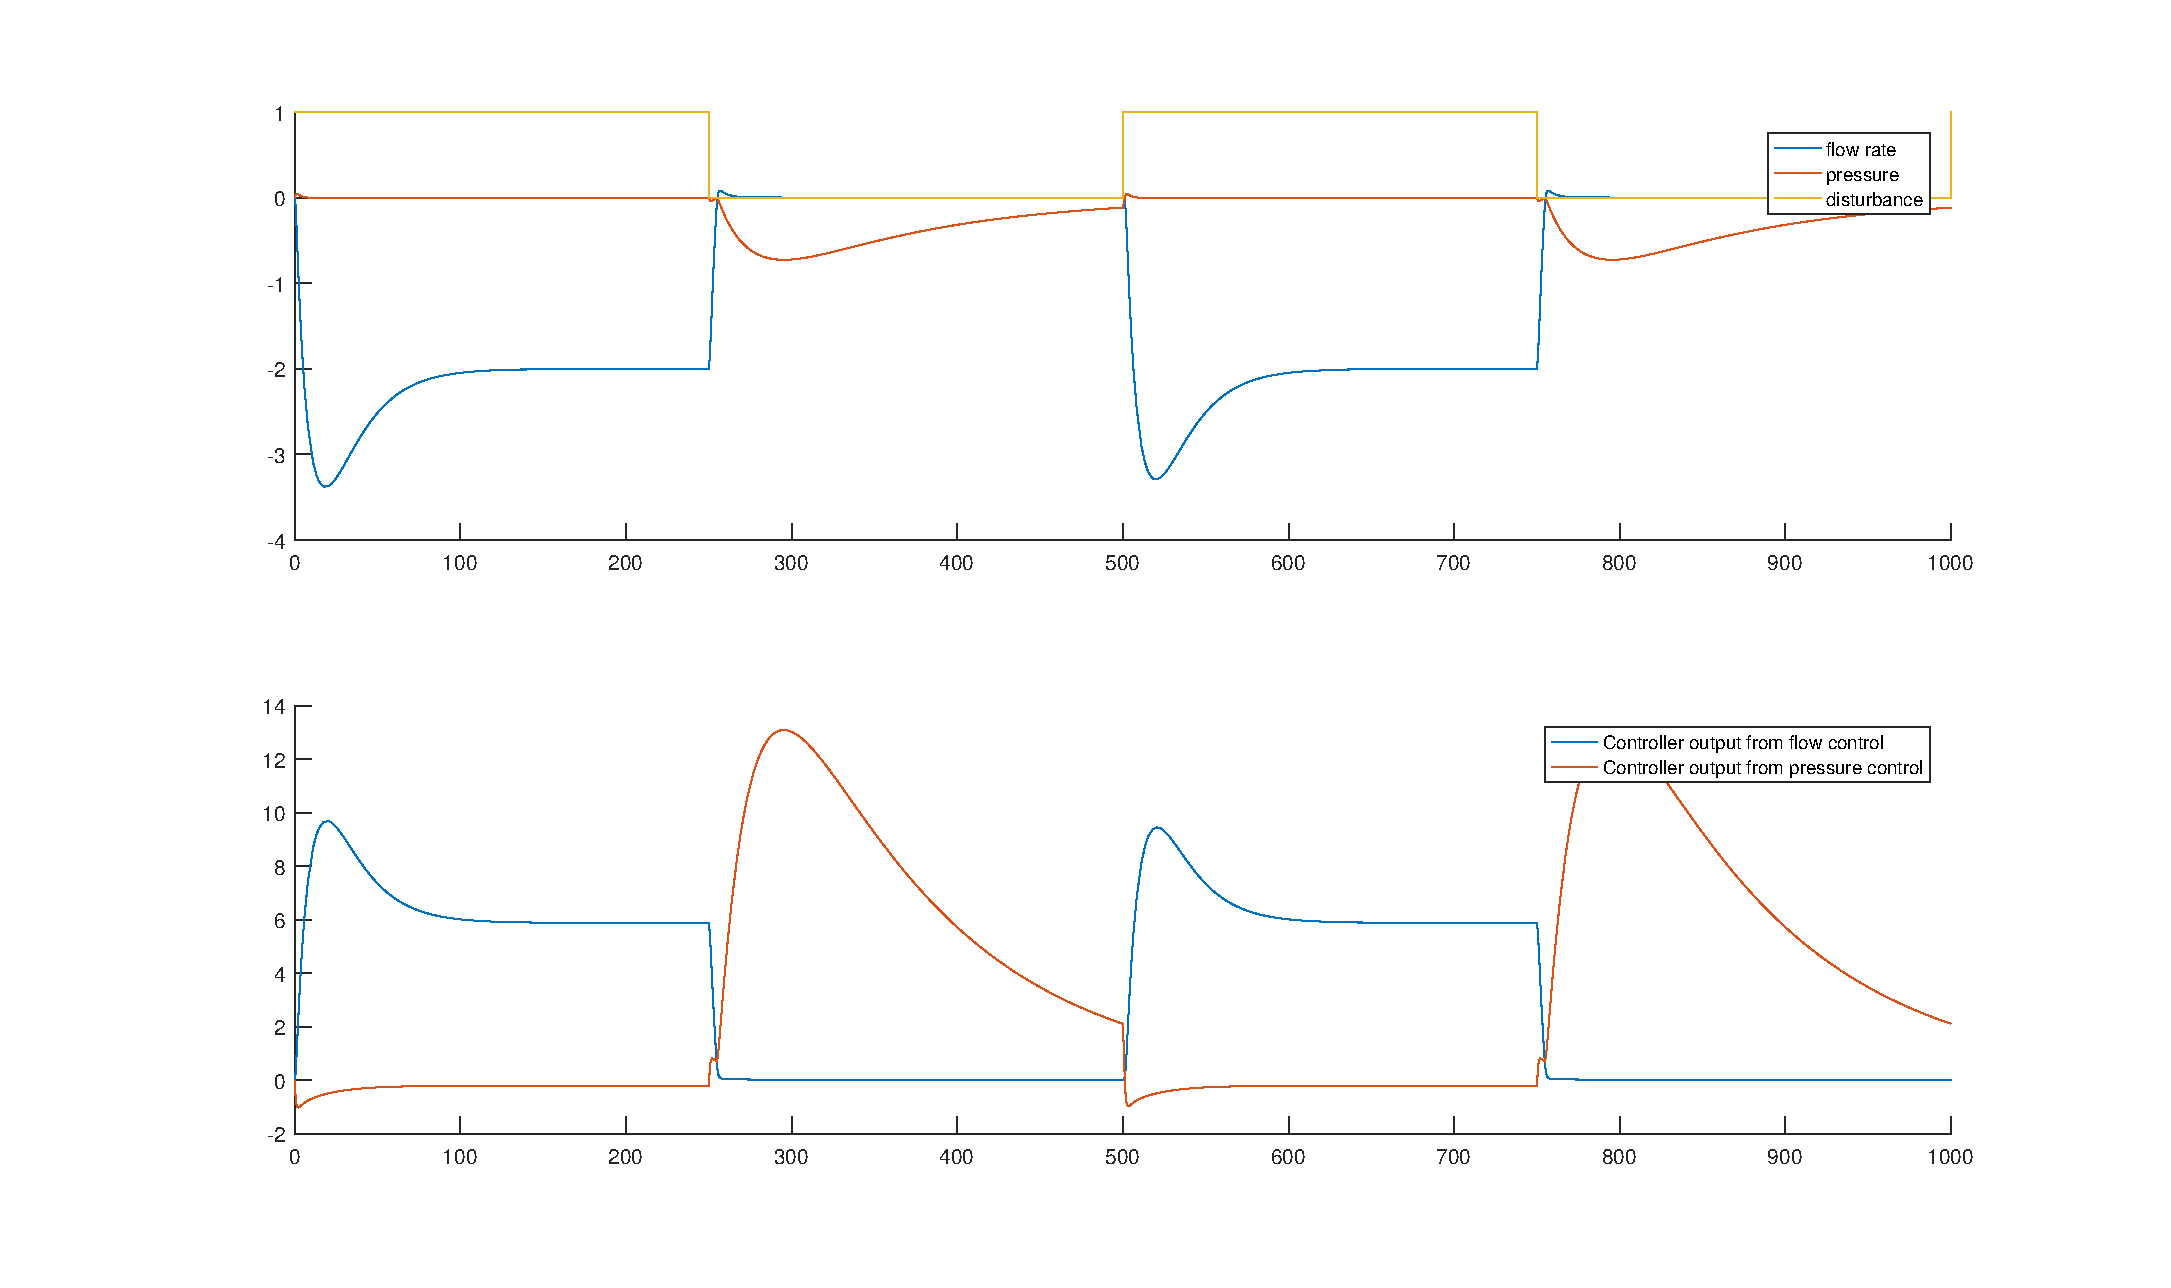
\includegraphics[width=0.9\textwidth]{fig/task2/2c_with_antiwindup_new.eps}
	\caption{System and controller output with anti-windup}
	\label{fig:2cwith}
\end{figure}

\end{document}